\chapter{Reducibility}

\lecture{11}{2025-12-1}{}

\begin{prev}
    \[
        A_{\text{TM}} \text{ is undecidable.}
    \]
\end{prev}

\vspace{1em}

We want to prove that other languages are undecidable. We can do a technique called \red{\textbf{reducibility}}.

\section{Reducibility}

\begin{definition}[reduction]
    Let $A$ and $B$ be languages. We say that $A$ is \textbf{mapping reducible} to $B$, written $A \leq_m B$, if there exists a computable function $f: \Sigma^* \to \Sigma^*$ such that for every $w \in \Sigma^*$,
    \[
        w \in A \iff f(w) \in B.
    \]
    The function $f$ is called a \textbf{reduction} from $A$ to $B$. Which means the converting process from an instance of problem $A$ to an instance of problem $B$, and $B$ can be used to solve $A$.
\end{definition}

\begin{theorem}
    If $A \leq_m B$ \[
        B \text{ is decidable } \implies A \text{ is decidable.}
    \]
    and 
    \[
        A \text{ is undecidable } \implies B \text{ is undecidable.}
    \]
\end{theorem}

\subsection{$E_{\text{TM}}$ is Undecidable}

\begin{eg}
    Consider the language
    \[
        E_{\text{TM}} = \{\langle M \rangle \mid M \text{ is a TM and } L(M) = \emptyset \}.
    \]
\end{eg}
\vspace{1em}

Assume $E_{\text{TM}}$ is decidable. We can get a decider $R$ for $E_{\text{TM}}$. From this, we can construct a decider $S$ for $A_{\text{TM}}$ as follows:
\begin{itemize}
    \item On input $\langle M, w \rangle$, where $M$ is a TM and $w$ is a string:
    \begin{enumerate}
        \item Construct a new TM $M_1$ as follows:
        \[
            L(M_1) = \emptyset \iff M \text{ does not accept } w \tag{1}
        \]
        \item Run $R$ on input $\langle M_1 \rangle$.
        \item If $R$ accepts, then reject. If $R$ rejects, then accept.
    \end{enumerate}
\end{itemize}
This construction is valid because of (1). Thus, if we had a decider for $E_{\text{TM}}$, we could construct a decider for $A_{\text{TM}}$. But we know that $A_{\text{TM}}$ is undecidable, so our assumption that $E_{\text{TM}}$ is decidable must be false. Therefore, $E_{\text{TM}}$ is undecidable.

\begin{note}
    $M_1$ takes input $x$ and have 
    \begin{enumerate}
        \item If $x \neq w$, then reject.
        \item If $x = w$, run $M$ on input $w$ and accept if $M$ accepts $w$.
    \end{enumerate}
    Clearly, \[
        L(M_1) = \emptyset \text{ or } \{w\}
    \]
    We see that \[
        \begin{cases}
            M \text{ accepts } w & \implies L(M_1) = \{w\} \neq \emptyset \\
            L(M_1) \neq \emptyset & \implies M \text{ accepts } w
        \end{cases}
    \]
    Thus, condition (1) holds.
\end{note}

\subsection{REGULAR$_{\text{TM}}$ is Undecidable}

\begin{eg}
    Consider the language
    \[
        \text{REGULAR}_{\text{TM}} = \{\langle M \rangle \mid M \text{ is a TM and } L(M) \text{ is a regular language} \}.
    \]
\end{eg}

As before, assume this language is decidable and has a decider $R$. We can construct a decider $S$ for $A_{\text{TM}}$ as follows:
\begin{itemize}
    \item On input $\langle M, w \rangle$, where $M$ is a TM and $w$ is a string:
    \begin{enumerate}
        \item Construct a new TM $M_2$ recognize: \[
            \begin{cases}
                \text{a regular language} & \text{if } M \text{ accepts } w \\
                \text{a non-regular language} & \text{if } M \text{ rejects } w
            \end{cases} \tag{1}
        \]
        \item Run $R$ on input $\langle M_2 \rangle$.
        \item If $R$ accepts, then accept. If $R$ rejects, then reject.
    \end{enumerate}
    \item Then we get $S$ \[
        \begin{cases}
            S \text{ accepts } & \text{if } M \text{ accepts } w \\
            S \text{ rejects } & \text{if } M \text{ rejects } w
        \end{cases}
    \]
    which is a decider for $A_{\text{TM}}$. Combining the $R$ and $M_2$ we can get a decider for $A_{\text{TM}}$. Getting a contradiction. Thus, REGULAR$_{\text{TM}}$ is undecidable.
\end{itemize}

\begin{note}
    $M_2$ recognizes the language \[
        L(M_2) = \begin{cases}
            \Sigma^* & \text{if } M \text{ accepts } w \\
            \{0^n1^n \mid n \geq 0\} & \text{if } M \text{ rejects } w
        \end{cases}
    \]
    We know that $\Sigma^*$ is regular and $\{0^n1^n \mid n \geq 0\}$ is not regular. Thus, condition (1) holds.\\
    
    The implementation of $M_2$ on input $x$ is as follows:
    \begin{enumerate}
        \item If $x$ is in the form $0^n1^n$, then accepts.
        \item If $x$ is not in the form $0^n1^n$, then simulate $M$ on input $w$, and accept if $M$ accepts $w$.
    \end{enumerate}
\end{note}

\subsection{EQ$_{\text{TM}}$ is Undecidable}

\begin{eg}
    Consider the language
    \[
        EQ_{\text{TM}} = \{\langle M_1, M_2 \rangle \mid M_1, M_2: \text{ TM},\ L(M_1) = L(M_2) \}. 
    \]
\end{eg}
\vspace{1em}

Assume $EQ_{\text{TM}}$ is decidable. We can get a decider $R$ for $EQ_{\text{TM}}$. From this, we can construct a decider $S$ for $E_{\text{TM}}$ as follows:
\begin{itemize}
    \item On input $\langle M \rangle$, where $M$ is a TM:
    \begin{enumerate}
        \item Running $R$ on input $\langle M, M_{\emptyset} \rangle$, where $M_{\emptyset}$ is a TM such that \[
            L(M_{\emptyset}) = \emptyset.
        \]
        \item If $R$ accepts, then accept. If $R$ rejects, then reject.
    \end{enumerate}
\end{itemize}

This construction is valid because \[
    L(M) = \emptyset \iff L(M) = L(M_{\emptyset}).
\] Thus, if we had a decider for $EQ_{\text{TM}}$, we could construct a decider for $E_{\text{TM}}$. But we know that $E_{\text{TM}}$ is undecidable, so our assumption that $EQ_{\text{TM}}$ is decidable must be false. Therefore, $EQ_{\text{TM}}$ is undecidable

\section{Computation Histories}

\begin{definition}
    $M$ is a TM and $w$ is an input string. An accepting \textbf{computation history} of $M$ on $w$ is \[
        C_1, C_2, \ldots, C_l
    \]
    where
    \begin{itemize}
        \item $C_1$ is the start configuration of $M$ on input $w$,
        \item $C_l$ is an accepting configuration, and
        \item for each $i$, $C_i$ legally yields $C_{i+1}$.
    \end{itemize}
\end{definition}

\begin{note}
    A rejection computation history is defined similarly, except that $C_l$ is a rejecting configuration. If $M$ loops on input $w$, then there is no computation history of $M$ on $w$.
\end{note}

\begin{remark}
    Deterministic TM has at most one (maybe reject or loop) computation history on input $w$, while a nondeterministic TM may have many computation histories on input $w$.
\end{remark}

\newpage

\subsection{Linear Bounded Automata (LBA)}

\begin{definition}[LBA]
    A \textbf{linear bounded automaton} (LBA) is a TM with a tape of limited length. Specifically, for an input string of length $n$, the tape head is not allowed to move beyond the first $n$ cells on the tape. If the head tries to move right at the end of input, the head stays
\end{definition}

\begin{figure}[H]
    \centering
    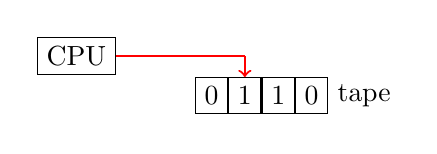
\begin{tikzpicture}[ampersand replacement=\&]
    \matrix 
    {
    \node[draw](0) {CPU}; \& [1cm] \& \node(1){}; \&\&\& \\
    \& \node[draw]{0}; \& \node[draw](a){1}; \& \node[draw]{1}; \& \node[draw]{0};  \& \node{tape};\\
    };
    \draw [-,red,thick] (0) -- (1.center) ;
    \draw [->,red,thick] (1.center) -- (a) ;
    \end{tikzpicture}
    \caption{Linear Bounded Automaton (LBA)}
\end{figure}

\begin{note}
    $A_{\text{DFA}}, A_{\text{CFG}}, E_{\text{DFA}}, E_{\text{CFG}}$ are all LBA-decidable.
\end{note}

\begin{theorem}
    LBA has a finite number of configurations.
\end{theorem}
\vspace{-1em}
\begin{proof}
    For an LBA $M$ with \[
        \begin{cases}
            q: \# \text{ states of } M = |Q| \\
            g: \# \text{ symbols of } M = |\Gamma|
        \end{cases}
    \]
    Then $M$ has at most \[
        q \cdot g^n \cdot n
    \]
    distinct configurations on an input of length $n$. Which is because:
    \begin{itemize}
        \item $q$ ways to choose the current state,
        \item $g^n$ ways to choose the content of the tape (only first $n$ cells matter),
        \item $n$ ways to choose the position of the tape head.
    \end{itemize}
    Thus, the total number of configurations is finite $qng^n$.
\end{proof}

\subsection{$A_{\text{LBA}}$ is Decidable}

\begin{eg}
    Consider the language
    \[
        A_{\text{LBA}} = \{\langle M, w \rangle \mid M: \text{ LBA that accepts } w \}.
    \]
\end{eg}

We only have to concern about is there loop or not, because if it halts then it either accepts or rejects. From the previous theorem, we know that an LBA has a finite number of configurations. Thus, if an LBA $M$ on input $w$ ever repeats a configuration, then $M$ will loop forever. 

\subsection{$E_{\text{LBA}}$ is Undecidable}

\begin{eg}
    Consider the language
    \[
        E_{\text{LBA}} = \{\langle M \rangle \mid M: \text{ LBA},\ L(M) = \emptyset \}.
    \]
\end{eg}
\vspace{1em}

The question of $M$ accepts $w$ can be solved by checking if $L(B) = \emptyset$, where $B$ is an LBA constructed from $M$ and $w$. Thus, we assume $E_{\text{LBA}}$ is decidable and has a decider $R$. We can construct a decider $S$ for $A_{\text{TM}}$ as follows:
\begin{itemize}
    \item On input $\langle M, w \rangle$, where $M$ is a TM and $w$ is a string:
    \item $B$ recognize all accepting computation histories of $M$ on input $w$.
    \[
        \begin{cases}
            M \text{ accepts } w & \implies L(B) \neq \emptyset \\
            M \text{ rejects } w & \implies L(B) = \emptyset
        \end{cases}
    \]
    \item Run $R$ on input $\langle B \rangle$.
    \item If $R$ accepts, then reject. If $R$ rejects, then accept.
\end{itemize}

The implementation of $B$ on input $x$ we check if it is an accepting computation history for $M$ on $w$. To be specifically, we check if $x$ is \[
    \# C_1 \# C_2 \# \cdots \# C_l \# \tag{1}
\]
and $C_1 \ldots C_l$ satisfies that 
\begin{itemize}
    \item $C_1$ is the start configuration of $M$ on input $w$,
    \item $C_l$ is an accepting configuration, and
    \item for each $i$, $C_i$ legally yields $C_{i+1}$.
\end{itemize}

\begin{figure}[H]
    \centering
    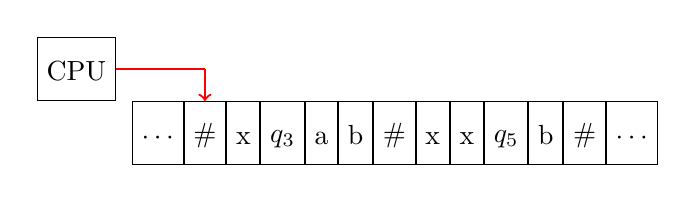
\begin{tikzpicture}[ampersand replacement=\&]
    \matrix[nodes={minimum height=8mm,text height=0.3cm}] 
    {
    \node[draw](0) {CPU}; \& [0.2cm] \& \node(1){}; \&\&\& \&\&\&\&\&\& \&\&\\
    \& \node[draw]{$\cdots$};
    \& \node[draw](a){\#};
    \& \node[draw]{x};
    \& \node[draw]{$q_3$};
    \& \node[draw]{a};
    \& \node[draw]{b};
    \& \node[draw]{\#};
    \& \node[draw]{x};
    \& \node[draw]{x};
    \& \node[draw]{$q_5$};
    \& \node[draw]{b};
    \& \node[draw]{\#};
    \& \node[draw]{$\cdots$};
    \\
    };
    \draw [-,red,thick] (0) -- (1.center) ;
    \draw [->,red,thick] (1.center) -- (a) ;
    \end{tikzpicture}
    \caption{Machine $B$ checking computation history}
\end{figure}

\begin{note}
    To check the conditions in (1), $B$ can scan through the input multiple times. Each time checking one of the conditions.
    \begin{enumerate}
        \item For the first condition, $B$ checks if $C_1$ matches $q_0 w$.
        \item For the last condition, $B$ checks if $C_l$ contains an $q_{\text{accept}}$.
        \item To check the middle condition, $B$ checks each pair $C_i$ and $C_{i+1}$ to see if $C_i$ legally yields $C_{i+1}$. This can be done by zigzags between $C_i$ and $C_{i+1}$. If this requires more space than the input length, but it is fine since the extra space for comparision is no more than $|\# C_1 \ldots \# C_l \#|$ which is finite.
    \end{enumerate}
\end{note}

\subsection{ALL$_{\text{CFG}}$ is Undecidable}

\begin{prev}
    \[
        E_{\text{CFG}} = \{\langle G \rangle \mid G: \text{ CFG},\ L(G) = \emptyset \} \text{ is decidable.}
    \]
\end{prev}

\begin{eg}
    Consider the language
    \[
        ALL_{\text{CFG}} = \{\langle G \rangle \mid G: \text{ CFG},\ L(G) = \Sigma^* \}.
    \]
\end{eg}
\vspace{1em}

It is impossible to check if $G$ gernerates all strings. We assume $ALL_{\text{CFG}}$ is decidable. We have \[
    G \text{ generates } \Sigma^* \iff M \text{ does not accept } w
\]
which is equivalent to
\[
    \begin{cases}
        G \text{ generates } \Sigma^* &\text{if } M \text{ does not accept } w \\
        G \text{ fails some strings} &\text{if } M \text{ accepts } w
    \end{cases}
\]
If we have a decider on $G$, then we can have a decider for $A_{\text{TM}}$. Getting a contradiction. If $M$ accepts $w$, we let $G$ fail to generate an accepting computation history of $M$ on $w$. i.e. $G$ generates all strings
\begin{enumerate}
    \item Not starting with $C_1$, \red{or}
    \item Not ending with an accepting configuration, \red{or}
    \item $C_i$ does not legally yield $C_{i+1}$ for some $i$.
\end{enumerate}

To construct such a CFG $G$, we can construct a PDA to nondeterministically checks three branches for the three requirements. The hardest one is the third branch, which can be done by pushing $C_i$ into the stack and popping from the stack to compare with $C_{i+1}$. To fix the order issue, we can push(pop) in this order \[
    \#\underbrace{\quad \rightarrow \quad}_{C_1}\#\underbrace{\quad \leftarrow \quad}_{C_2^R}\#
    \underbrace{\quad \rightarrow \quad}_{C_3}\#\underbrace{\quad \leftarrow \quad}_{C_4^R}\#
    \cdots\#\underbrace{\qquad}_{C_l}\#
\]